%\documentclass[12pt]{scrreprt}
\documentclass[12pt]{report} 

\setcounter{tocdepth}{3}
\setcounter{secnumdepth}{3}

% language may be romanian or english (default is english)
% type may be bachelor or master (default is bachelor)
\usepackage[language=english, type=bachelor]{style}

%\geometry{a4paper,top=2.5cm,left=3cm,right=2.5cm,bottom=2.5cm}
%in style
%controlling the appearance of your headers and footers
\usepackage{fancyhdr}
\usepackage{amssymb}
\usepackage{amsmath}
\pagestyle{fancy}
\lhead{}
\chead{}
\renewcommand{\headrulewidth}{0.2pt}
\renewcommand{\footrulewidth}{0.2pt}

\begin{document}

\specialization{[Sec\c tie]}	
\title{[Titlu lucrare]}					   
\author{[Nume student]}											
\supervisor{[Grad, titlu si nume coordonator]}				
				
\maketitle


\newpage
\thispagestyle{empty}
\mbox{}
\newpage
\pagenumbering{roman} 

\cleardoublepage
ABSTRACT
\vspace{0.5cm}	
\hrule
\vspace{0.5cm}	
%\cleardoublepage

Abstract: un rezumat \^{i}n limba englez\u{a} cu prezentarea, pe scurt, a con\c{t}inutului pe capitole, pun\^{a}nd accent pe contribu\c{t}iile proprii \c{s}i originalitate



\tableofcontents


\newpage
\pagenumbering{arabic}

\chapter{Introduction}

%\chapter*{Introduction}
\label{intro}

\par Introducere: obiectivele lucrarii si descrierea succinta a capitolelor, prezentarea temei, prezentarea contributiei proprii, respectiv a rezultatelor originale si mentionarea (daca este cazul) a sesiunii de comunicari unde a fost prezentata sau a revistei unde a fost publicata.
%\addcontentsline{toc}{chapter}{Introducere}
%\addcontentsline{toc}{chapter}{Introduction}

\chapter{Optical Character Recognition}
\label{chap:ch3}


\par Lorem ipsum dolor sit amet

\section{Problem overview}
\label{sec:ch3sec1}

\section{Printed/handwritten text recognition}
\label{sec:ch3sec1}

\section{Offline recognition. Online recognition}

\section{Motivation of AI-based solutions}
\label{sec:ch3sec1}

\chapter{Neural networks. General notions}
\label{chap:ch3}






\section{A short historic insight}
\label{sec:ch3sec1}
\par The concept of artificial intelligence is almost as old as modern computing. Initially started as a product of fantasy by science-fiction authors like Isaac Asimov, the advancement of technology revealed the true potential of computing machines. Alan Turing, the one who in 1940's broke the German Enigma code during World War II, has formulated the famous Turing test, meant to define machine intelligence based on the incapacity of a human actor to distinguish whether an entity is a human or a robot while interacting with it. Eventually, more formal definitions of machine learning arose by the work of John McCarthy, Marvin Minsky, Allen Newell, Herbert Simon and others. AI research has been flourished until the 1970's when it was met with the computing power limitations of that time. It was not until the 1980's when governments and agencies restarted to fund AI projects, but significant progress started to cristalize once the hardware became more capable, improved algorithms came to light and 
researchers performed a shift of mindset from expert systems, rules in decision making, to considering approaches based on probabilities which opened up the way to neural networks and what we know today as deep learning. \cite{BriefHistoryOfAI}

\section{Machine learning. Theoretical foundations}
\label{subsec:ch3sec2}
\input{chapters/sections/3_2_MachineLearningTheory}

\subsection{Vectors. Matrices. Tensors. Operations}
\label{subsec:ch3sec2subsec1}
\par A vector is a tool that enables processing of multiple quantities at once. \cite{IntroVec} Let $x_1, x_2, \ldots x_n \in \mathbb{K}$ be $n$ values in a field $(\mathbb{K},+,\cdot)$. Using these values we can build an $n$-dimensional vector $\mathrm{x}$ described as a tuple $\mathrm{x} = (x_1, \ldots,x_n)\in\mathbb{K}^n$. In the following we consider $\mathbb{K} = \mathbb{R}$ and highlight the most usual vector properties and operations.
The addition of two vectors $\mathrm{x}$ and $\mathrm{y}$ in $\mathbb{R}^n$ is defined as the vector obtained from summing each component of one vector with its counterpart from the other vector:
$$\mathrm{x}+\mathrm{y} = (x_1,\ldots,x_n)+(y_1,\ldots,y_n)=(x_1+y_1,\ldots,x_n+y_n).$$
Obviously, vector addition is commutative: $\mathrm{x}+\mathrm{y}=\mathrm{y}+\mathrm{x} \ \forall \mathrm{x},\mathrm{y}\in\mathbb{R}^n $, and associative: $(\mathrm{x}+\mathrm{y})+\mathrm{z}=\mathrm{x}+(\mathrm{y}+\mathrm{z}) \ \forall \mathrm{x},\mathrm{y},\mathrm{z}\in\mathbb{R}^n $. The vector $\mathrm{0}=(0,...0)\in \mathbb{R}^n$ is the neutral element with respect to addition ($\mathrm{x}+\mathrm{0}=\mathrm{x}\ \forall \mathrm{x} \in\mathbb{R}^n $) and for each vector $\mathrm{x}$ there exists an inverse vector $-\mathrm{x}=(-x_1,\ldots,-x_n)$ such that $\mathrm{x}+(-\mathrm{x})=\mathrm{0}$. \cite{IntroVec}

Let $\alpha\in\mathbb{R}$ be a scalar and $\mathrm{x}\in\mathbb{R}^n$ a vector. The vector $\alpha\mathrm{x}=(\alpha x_1,\ldots,\alpha x_n)$ is called the 
product of the vector $\mathrm{x}$ with the scalar $\alpha$. The usual properties of multiplication hold: \cite{IntroVec}
\begin{itemize}
\item associativity: $(\alpha\beta)\mathrm{x} = \alpha(\beta\mathrm{x}), \beta\in \mathbb{R}$;
\item identity: $\mathrm{1}\mathrm{x}=\mathrm{x}$;
\item distributivity of vector: $(\alpha+\beta)\mathrm{}{x}=\alpha\mathrm{x}+\beta\mathrm{x}$
\item distributivity of scalar:
$\alpha(\mathrm{x}+\mathrm{y})=\alpha\mathrm{x}+\alpha\mathrm{y}, \mathrm{y}\in\mathbb{R}^n$
\end{itemize} 

\par Given a vector $\mathrm{x}\in\mathbb{R}^n$, we define the magnitude of the vector $|\mathrm{x}|$ to be the euclidean norm of its components:
$$ |\mathrm{x}| = \sqrt{(x_1^2 + \ldots + x_n^2)}. $$
It can be easily verified that for $\alpha\in\mathbb{R}$, $|\alpha \mathrm{x}|=|\alpha|\cdot|\mathrm{x}|$ \cite{IntroVec}. A vector with magnitude $1$ is called unit (or direction) vector. 

\par The interesting part arises when we try to imagine the product of two vectors. Some popular definitions are scalar and vector products. We are focusing on the scalar product, as it is more relevant for the current work. There are two useful formulations of the scalar product $\mathrm{x}\cdot\mathrm{y}$ (also called inner, or dot product \cite{IntroVec}) of two vectors $\mathrm{x},\mathrm{y}\in\mathbb{R}^n$. One of them is defined in function of their components:
$$\mathrm{x}\cdot\mathrm{y}=\sum_{i=1}^{n}{x_i y_i}=x_1 y_1 + \ldots + x_n y_n.$$
The other one emerges from the geometric interpretation of the scalar product as being the length of the projection of one vector to the other:
$$\mathrm{x}\cdot\mathrm{y} = |\mathrm{x}||\mathrm{y}| \cos{\angle{(\mathrm{x},\mathrm{y})}}.$$
This last relation, stripped of its geometric meaning, inspires one of the applications of the scalar product as an expression of similarity between two vectors, describing how much one diverges from another by measuring the angle between them. \cite{cossim}

\par We call a matrix $A \in\mathcal{M}_{m,n}(\mathbb{R}), m,n\in\mathbb{N}^\star$ a collection of $m \times n$ real scalars displayed in a tabular grid consisting of $n$ rows and $m$ columns:
$$ A = \begin{bmatrix}
    a_{11}       & a_{12} & a_{13} & \dots & a_{1m} \\
    a_{21}       & a_{22} & a_{23} & \dots & a_{2m} \\
    \hdotsfor{5} \\
    a_{n1}       & a_{n2} & a_{n3} & \dots & a_{nm}
\end{bmatrix},$$
where the element $a_{i j}$ is placed at row $i$, column $j$. \cite{LinAlSchaum}
The short notation of the matrix $A$ using its elements $a_{i j}, 1 \leq i \leq n, 1 \leq j \leq m$ is $A=(a_{i j})_{1 \leq i \leq n, 1 \leq j \leq m }$.
Note that a vector can be visualized as a matrix where one of the dimensions is equal to $1$. Hence, the vector $(x_1,\ldots,x_n)\in\mathbb{R}^n$ can be viewed either as a 
one-line matrix $ \begin{bmatrix} x_{1} & x_{2} & \dots & x_{n}  \end{bmatrix}\in \mathcal{M}_{1,n}(\mathbb{R}) $, or as a one-column matrix
$ \begin{bmatrix} x_{1} & x_{2} & \dots & x_{n}  \end{bmatrix}^T = \begin{bmatrix} x_{1} \\ \vdots \\ x_{n}  \end{bmatrix}^T \in \mathcal{M}_{n,1}(\mathbb{R}) $.

\par The matrix addition and scalar multiplication are defined analogously to the vector operations and share the same properties \cite{LinAlSchaum}. For matrices $A=(a_{i j}),B=(b_{i j}) \in\mathcal{M}_{m,n}(\mathbb{R})$ and scalar $\alpha \in \mathbb{R}$, we have:
\begin{itemize}
\item $A+B = (a_{i j} + b_{i j})_{(i,j)\in\mathbb{R}^2 \cap ([1,n]\times[1,m])}$;
\item $\alpha A = (\alpha a_{i j})_{(i,j)\in\mathbb{R}^2 \cap ([1,n]\times[1,m])}$.
\end{itemize} 

\par Now let's consider two matrices $A \in\mathcal{M}_{m,n}(\mathbb{R}), B \in\mathcal{M}_{n,p}(\mathbb{R}), n,m,p \in \mathbb{N}^\star$. The product of the two matrix is the matrix $C = AB \in \mathcal{M}_{m,p}$, where
$$c_{i j} = \sum_{k=0}^{m} {a_{i k} b_{k j}}. $$
Note the analogy with the vectors' scalar product. In fact, when $m=p=1$, the matrix multiplication between a column vector and a row vector produces in fact the scalar product of these two vectors.

\par So far we have considered a vector to be an ordered collection of scalars, and a matrix to be a stacked collection of vectors. We can extend this process and infer the concept of stacked matrices of same type to form a 3-dimensional structure of scalars, and we can continue like that on higher dimensions. We will refer to these structures as tensors. For matters of simplicity, we will skip over some rigorous mathematical aspects of tensors \cite{TensorsPorat_2014} like variance and emphasize on the more intuitive properties that are useful in this work from a computational point of view. We therefore consider a tensor to be a collection of scalars with multidimensional index access. Let $n$ be the number of dimensions of the tensor and $d_1, d_2, \ldots, d_n \in \mathbb{N}$ the length of each dimension. The number $n$ is called the rank of the tensor, while the tuple $d=(d_1,\ldots,d_n)$ is the shape of the tensor. For a tensor $t$ of rank $n$ and dimension $d$, we note $t_{i_1 i_2 \ldots i_n}$ the component contained at indices $1 \leq i_j \leq d_j, j= \overline{1,n}$. When $n=0$, we call it a shapeless tensor, and it roughly behaves like a scalar value. We introduce the notation $\mathcal{T}_{n}(d)=\{t \ | \ t \ \mathrm{is} \ a \ \mathrm{tensor} \ \mathrm{of} \ \mathrm{rank} \ n \ \mathrm{and} \ \mathrm{shape} \ d, d=(d_1,...,d_n)\}$ the set of $d$-shaped tensors, and $\mathcal{D}(d)=\prod_{k=1}^{n}{[1,d_k]}\times \mathbb{N}^n$ the set of all possible indices tuples corresponding to shape $d$. We use the term "axis $k$ of a rank $n$ tensor", $1 \leq k \leq n$, to refer the the $k$-th dimension of its shape. For example, in a matrix trated as a rank 2 tensor, axis 1 names the rows indices, while axis 2 describes the column indices. The length of an axis $k$ is $d_k$, the largest possible index value of that dimension. In the following, we will describe some commonly used operations with tensors. \cite{D2l}

\par RESHAPE!!!!!!!!!!!!

\par Element-wise operations are performed on tensors of the same shape $d$. Considering an operator $ \bullet : \mathbb{R} \times \mathbb{R} \rightarrow \mathbb{R}$ defined on scalar pairs, We can extend its functionality on tensors $ \bullet_T : \mathcal{T}_{n}(d) \times \mathcal{T}_{n}(d) \rightarrow \mathcal{T}_{n}(d)$, $A \bullet_T B = C$, where $c_i = a_i \bullet b_i, i \in \mathcal{D}(d)$. The operator $\bullet$ can represent any usual arithmetic operation. In particular, when $\bullet=\cdot$ real multiplication operator and $n=2$, the operator $\bullet_T = \circledcirc$  is called the Hadamard product \cite{D2l}, the element by element multiplication performed on matrices, $A \circledcirc B = (a_{i j} b_{i j})_{(i,j)\in \mathcal{D}(d)}$. Generalizing further, we can make the operator $\bullet_T$ allow arguments of different shapes: $\bullet_T : \mathcal{T}(d_1) \times \mathcal{T}(d_2)\leftarrow \mathcal{T}(d_r)$. By choosing, for example, $d_1=()$, $a \bullet B$ is an operation between a scalar and a tensor and can be viewed as streaming the scalar value to each component of the tensor. It is virtually equivalent to creating as many copies of the scalar $a$ as the components count of tensor $B$ and placing them in the same shape as the tensor. Thus, $a \bullet_T B$ reduces to calculating $A \bullet_T B$, where $A=(a)_{i\in \mathcal{D}(d_2)}$. A similar approach can be performed for $d_1=(1)$. Let's consider now two arbitrary shapes $d_1$ and $d_2$ of the same rank and for each axis $k$, either $d_{1 k} = d_{2 k}$ or one of $d_{1 k}$ for ${d_{2 k}}$ is equal to ${1}$. Therefore, we are building the output of $A \bullet_T B$ as the tensor $C \in \mathcal{T}(d_r)$ with $d_r=(\max{\{d_{1 i}, {d_{2 i}\}}})_{i=\overline{1,n}}, c_{i_1 \ldots i_n} = a_{\theta_a} \bullet b_{\theta_b}$, where $\theta_a = (\min{(i_k, d_{1 k})})_{k=\overline{1,n}}$ and $\theta_b = (\min{(i_k, d_{2 k})})_{k=\overline{1,n}}$. If $d1$ and $d2$ are of different shapes, one can consider reshapind the tensor of lower rank to by prepending axis of length 1 until it reaches the same rank as the other tensor and applying the steps above. This process is known as tensor broadcasting. 

\subsection{Linear regression. Loss functions. Activation functions}
\label{subsec:ch3sec2subsec2}
\par The usual neural network problem formulation involves predicting values based on existing observations. When the output domain is a continuous space, it becomes a regression problem. Prediction of discrete values, on the other hand, is called classification \cite{D2l}.

\par In the following, we consider a independent variable $\mathrm{x}$ of input features and some targets $\mathrm{y}$ dependent on $\mathrm{x}$ in an approximately linear way. 
\par In its simplest form, $\mathrm{x}$ is unidimensional variable and dependence between $\mathrm{x}$ and $\mathrm{y}$ is approximated by the relation $\mathrm{y}=\alpha \mathrm{x} + \beta$. Our aim is to find $\alpha$ and $\beta$ that best fit a set of $n$ observations of the behavior of $y^(i)$ with respect to the input $x^(i)$, $(x^{(i)}, y^{(i)})_{i=\overline{1,n}}$. We are trying to find the optimal parameters that minimize the error $|y^{(i)}-\alpha x^{(i)} - \beta|$ across all observations --- see Figure \ref{FigLinReg2D}.

\par Let's define the cummulative error $err(\alpha, \beta)=\sum_{i=1}^{n}{\left| \alpha x^{(i)}+\beta-y^{(i)} \right| ^2}
= \sum_{i=1}^n{(x_{(i)})^2} \alpha^2 + n \beta^2 + \sum_{i=1}^n{(y_{(i)})^2} 
+ 2\sum_{i=1}^n{x_{(i)}} \alpha\beta - 2\sum_{i=1}^n{x_{(i)}}{y_{(i)}} \alpha 
- 2\sum_{i=1}^n{y_{(i)}} \beta$. The function reaches its critical point in $(\alpha^\star, \beta^\star)$ which cancels the gradient:
$\nabla err = 0 \leftrightarrow (\frac{\partial err}{\partial \alpha}, \frac{\partial err}{\partial \beta})=0 \leftrightarrow$
$$
\begin{cases}
2\sum_{i-1}^n{(x^{(i)})^2}\alpha +2\sum_{i-1}^n{x^{(i)}}\beta - 2\sum_{i-1}^n{x^{(i)}y^{(i)}} = 0 \\
2\sum_{i-1}^n{x^{(i)}}\alpha + 2 n \beta - 2\sum_{i-1}^n{y^{(i)}} = 0.
\end{cases}
$$
The system can be written in matrix form as 
$$
\begin{bmatrix}
\sum_{i-1}^n{(x^{(i)})^2} & \sum_{i-1}^n{x^{(i)}} \\
\sum_{i-1}^n{x^{(i)}} & n
\end{bmatrix} \begin{bmatrix}
\alpha \\ \beta
\end{bmatrix} = \begin{bmatrix}
    \sum_{i-1}^n{x^{(i)}y^{(i)}} \\
    \sum_{i-1}^n{y^{(i)}}
\end{bmatrix}.
$$
With the notation $X^T=\begin{bmatrix} x^{(1)} & x^{(2)} &  \dots & x^{(n)} \\ 1 & 1 & \dots & 1 \end{bmatrix}$ and $Y^T=\begin{bmatrix}y^{(1)} & y^{(2)} & \dots & y^{(n)} \end{bmatrix}$, we are left with the nice equation $X^T X \begin{bmatrix}
\alpha \\ \beta \end{bmatrix} = X^T Y$, whose solution is 
$$\begin{bmatrix}\alpha \\ \beta \end{bmatrix} = (X^T X)^{-1} X^T Y,$$
The described approach is called the Least Square Method (LSM) \cite{linregreview}, which focuses on minimizing the square of the fitting errors for each data in the system.

\begin{figure}[htbp]
	\centering
		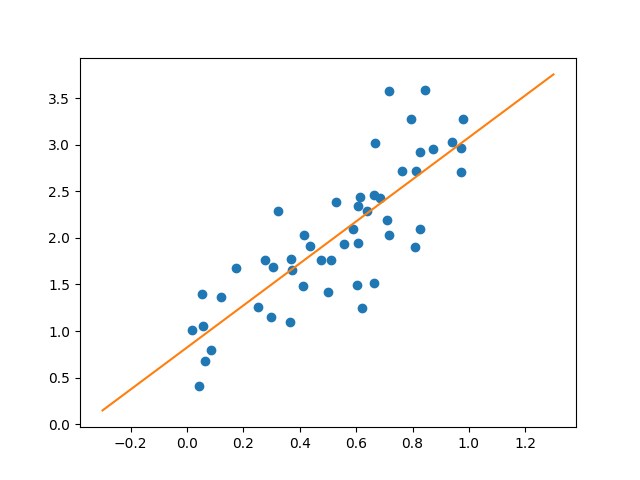
\includegraphics[scale=0.5]{figures/lin_reg_2d.png}
	\caption{Linear regression example in 2D space, with $\alpha=2, \beta=1$}
	\label{FigLinReg2D}
\end{figure}

This method can be extended to multivariate linear regression \cite{linregreview}, where each observation $x^{(i)}$ consists of multiple features $x^{(i)}_1,\ldots,x^{(i)}_m$ and we are finding the values $\beta=(\beta_0,\ldots,\beta_m)$ that minimize $\beta_0 + \beta_1 x^{(1)}+\ldots+\beta_m x^{(m)}$. By taking $X^T=\begin{bmatrix}
x^{(1)}_1 & x^{(2)}_1 & \ldots & x^{(n)}_1 \\
\vdots & \vdots & \ddots & \vdots \\
x^{(1)}_m & x^{(2)}_m & \ldots & x^{(n)}_m \\
1 & 1 & \ldots & 1 
\end{bmatrix}$, the previous relation $\beta = (X^T X)^{-1}X^T Y$ holds true, as long as $ (X^T X)$ is invertible. A singular matrix would suggest that the variables $x$ may not be linearly independent. There may exist a hyperplane of lower order that contains them and allows for infinite regression possibilities (for example, all $x^{(i)}$ are located in the same point in a 2D space through which can pass an infinity of lines, or on a line in 3D space).

Obviously the linear regression is designed to only find almost linear relations between data. One famous example is the XOR function \ref{FigXorLin}. Attempting to obtain a prediction by linear regression would lead to a function that uniformly averages the expected output values, and thus it is said that the values are linearly inseparable \cite{xorexample}. Another drawback of this method is the requirement to compute the inverse of the matrix in order to solve the system, which can prove computationally expensive. This opens up the door for faster iterative and potentially more general approaches, like the gradient descent, which will be discussed later in this thesis.

\begin{figure}[htbp]
	\centering
		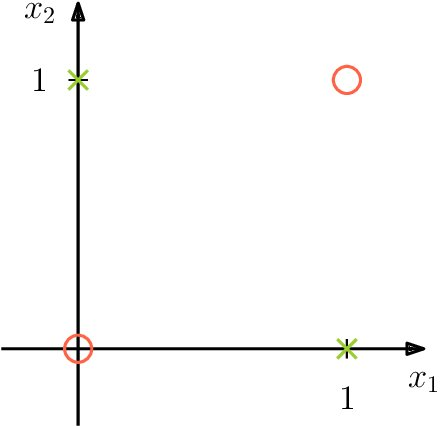
\includegraphics[scale=1]{figures/xor_lin.jpg}
	\caption{The XOR function cannot be predicted by a linear regression model \cite{xorexample}}
	\label{FigXorLin}        
\end{figure}




\par However, we can derive from this method a recurrent aspect in optimization problems: the concept of loss function. A loss function is a function $\mathcal{L}(\mathrm{y}, \mathrm{y^\star})$ destined to 
measure the reliability of our prediction by comparing the real reference values with the predicted output. Minimizing the loss function is associated with a better prediction \cite{losssurvey}. The loss function 
$err$ used by LSM is an example of loss function. Other common regression loss functions are Mean Absolute Error (MAE) or $\mathcal{L}_1$ loss, $\mathcal{L}_{MAE} = \frac{1}{n}\sum_{i=1}^n{\left| y_i - y_i^\star \right|}$, the Mean Squared Error (MSE), or $\mathcal{L}_2$ loss, $\mathcal{L}_{MAE} = \frac{1}{n}\sum_{i=1}^n{\left| y_i - y_i^\star \right|^2}$, or the Huber loss, which combines the previous two functions by exploiting the fact that MAE is good for large errors and MSE is suitable for smaller residuals \cite{losssurvey}.


\par A widely adopted approach to fight linearity in predictions is to pass the outputs $\mathrm{y}^\star$ to a (non-linear) function called an activation function \cite{activsurvey}. They are meant to increase the ability of the solution to find more sophisticated relations in the processed data. Their role will be emphasized when we will talk about neural network layers. By chaining two linear prediction functions $f_1$ and $f_2$ with no activation (or, synonymously, linear activation), the result $f_1 \circ f_2$ is also linear. However, by applying a non-linear activation $f_a$ to $f_1$ before plugging its results into $f_2$, the resulted application $f_1 \circ f_a \circ f_2$ is no longer linear in terms of the input $\mathrm{x}$. Table \ref{Activations} contains a list of popular activation functions \cite{activsurvey}.


\begin{table}[htbp]
\begin{center}
\begin{tabular}
{|p{120pt}|p{120pt}|}
\hline
 Name  &  Formula\\
\hline Tanh & $(e^{2x}-1)/(e^{2x}+1)$ \\ 
\hline ReLU & $\max(0, x)$ \\ 
\hline LeakyReLU & $ x, \text{if} \ x \geq 0, \text{else} \ \alpha x $ \\ 
\hline Sigmoid & $(1+e^{-x})^{-1}$ \\ 
\hline Swish & $x \cdot \textit{sigmoid}(x)$ \\ 
\hline
\end{tabular}
\end{center}
\caption{Common activation functions \cite{activsurvey}}
\label{Activations}
\end{table}

%\marginpar{\textcolor{green}{eu zic ca acestea sunt functii de activare (in tabelul 2.1, nu fc de loss)}} % solved (copy paste issues)
The choice for loss and activation functions is solely dependent on the problem \cite{losssurvey}. They can dictate the eligibility of the solution and convergence rate. Like LeakyReLU, most functions allow customizing their parameters (called hyperparameters) and in most machine learning frameworks come with multiple variants (like the scaled sigmoid, hard sigmoid etc.) \cite{activsurvey}, \cite{actfcomp}.

\subsection{Derivation. Differentiation. Backpropagation}
\label{subsec:ch3sec2subsec3}
\par Let $f:\mathbb{R}->\mathbb{R}$ a real function. We call derivative of $f$, the function $f'$ such that
$$f'(x) =\lim_{h\rightarrow 0}\frac{f(x+h)-f(x)}{h}.$$
Function $f$ is differentiable at $x$ if the limit in $f'$ exists. $f$ is differentiable on an interval $[a,b]$ if it is differentiable at any point in that interval. We can also use $\frac{df}{dx} = f'$ as a notation for the derivative \cite{D2l}.

\par We recall the fundamental properties of derivatives \cite{D2l}:
\begin{itemize}
\item $\frac{d}{dx}(cf) = c\frac{df}{dx}, c\in\mathbb{R}$;
\item $\frac{d}{dx}(f+g) = \frac{df}{dx} + \frac{dg}{dx}$;
\item $\frac{d}{dx}(fg) = \frac{df}{dx}g + f\frac{dg}{dx}$;
\item $\frac{d}{dx}(\frac{f}{g}) = \frac{\frac{df}{dx}g - f\frac{dg}{dx}}{g^2}$;
\item $\frac{d}{dx}(f(g)) = \frac{d(f(g))}{dg}\frac{dg}{dx}$ (chain rule)
\end{itemize}


\par Let's consider $f:\mathbb{R}^n\rightarrow \mathbb{R}$ a function of multiple variables. The partial derivative of $f$ with respect to the $i$-th argument is
$$\frac{\partial f}{\partial x_i} = \partial_{x_i}f = \lim_{h \rightarrow 0} \frac{f(x_1, \ldots,x_{i-1},x_i+h,x_{i+1},\ldots,x_n)-f(x_1, \ldots,x_{i-1},x_i,x_{i+1},\ldots,x_n)}{h}.$$ The function $\nabla_{\mathrm{x}}f:\mathbb{R}^n\rightarrow\mathbb{R}^n$,
$$\nabla_{\mathrm{x}}f(\mathrm{x}) = \begin{bmatrix} \partial_{x_1}f(\mathrm{x}) \ldots \partial_{x_n}f(\mathrm{x}) \end{bmatrix}^T $$
is called the gradient of $f$. All these definitions can be easily adapted to functions with multiple outputs \cite{D2l}.

\par As in machine learning we often meet the need to differentiate chains of composite functions, it is critical to remind the chain rule for multivariate derivatives. For a composite function $y(\mathrm{x})=f(u(\mathrm{x}))$, where $f:\mathbb{R}^m\rightarrow \mathbb{R}^q$ and $u:\mathbb{R^n}\rightarrow\mathbb{R^m}$, the derivative of $y$ with respect to $x_i$ is
$$\frac{\partial y}{\partial x_i} = \sum_{j=0}^m \frac{\partial y}{\partial u_j} \frac{\partial u_j}{\partial x_i}, $$
and therefore $\nabla_\mathrm{x}y = J_u(\mathrm{x}) \nabla_u{y}$, where $J_u$ is the Jacobian matrix of $\mathrm{u}$ \cite{D2l} \cite{damadi2023backpropagation}.

\par The chain rule constitutes the foundation of training AI models, because it provides a way to automatically perform differentiation. This operation fortunately is handled internally by the usual machine learning libraries. A complex function is converted into an operation flow graph, where nodes represent operations and edges illustrate dependencies. To graphically represent $f(g)$, one would draw a directed arc from node $g$ to node $f$. An input is pumped through the graph starting from $g$, and it is gradually transformed by the function residing at each node it visits. This process is called (forward) propagation. To obtain the gradient of the composite function, one would process the graph the reverse way starting from outputs and applying the gradients according to the chain rule, thus performing a backpropagation through the computational graph \cite{D2l}. The goal of backpropagation is to compute the gradients that will be used in adjusting the parameters of the prediction function by the optimizer algorithms \cite{damadi2023backpropagation}.




\subsection{Classification}
\label{subsec:ch3sec2subsec4}
\par The classification problem introduces the concept of labels. They are discrete values, usually numerical, that are predicted by a function $f:D\rightarrow L$, where $D$ is the input domain, and $L$ is a finite set of labels. However, this mathematical approach makes it struggling to optimize the objective function, due to the fact that $L$ is not a continuous set, so $f$ cannot be differentiable. We might want to assure the continuity of $f$. Even though various solution may be propose to this problem, like interpolating between the label values (like ${0,1}$ or ${-1,1}$ for binary classification), we will focus on the probabilistic approach of letting $L=\{ l | l=(l_1,\ldots,l_n)\in\mathbb{R}^{n}, l_1+\ldots+l_n=1, l_i\geq 0\}$ be a vector set whose components at position $i$ are interpreted as the probability of the input data to be of label $i$ \cite{D2l}. For $n=2$, we are faced with a binary classification problem. A multi-class classification can be reduced to a binary classification problem by choosing the output form to be a list of $\mathbb{R}^2$ categorical vectors, each one representing a confidence factor of a certain label to be a true class of the analyzed data. This last model is also suitable for multi-label classification, the type of problem where an input can belong to one or more classes \cite{D2l}.
\par The last step in such a classification approach is collapsing the continuous output to a discrete label value. As we have observed, for a probabilistic model the discrete output would be the index of the label that appears with the highest probability. In case of a general continuous model, some threshold would apply to obtain the closest integer label according to problem-specific chosen conditions.


\subsubsection{Classification losses}
\label{subsubsec:ch3sec2subsec4subsubsec1}

\par In other words, classification problems can be therefore transformed into regression problems by relaxing the output constraints. Intuitively, instead of requiring the predicted value $\mathrm{y}^\star$ to be either a fixed $0$ or $1$, we can allow the function to predict continuous values based on which one could eventually make a final decision regarding the predicted class. A simple example of reasoning would be to consider that $\mathrm{x}$ for which $\mathrm{y}^\star=f(\mathrm{x}) \geq 0.5$ are more likely to have their corresponding output $\mathrm{y}=1$ than of class $\mathrm{y}=0$. Such $y^\star$ are called logits. Furthermore, this "likeliness" idea conduces to a more formal description that can be also generalized to multi-label classification. Our function will try to predict a vector of probabilities of the same length as the number of classes where the probabilities add up to 1 \cite{losssurvey}. The prediction function is trying to raise the probability of the real labels while lowering the potential for a mistaken guess. A remarkable type of classification loss is the cross entropy loss that takes advantage of the properties of probabilities distributions: $\textit{crossentropy}(\mathrm{y}, \mathrm{y^\star}) = -\sum_{i=0}^n{\mathrm{y_i} \log{\mathrm{y_i^\star}}}$ \cite{losssurvey}.

\begin{table}[htbp]
\begin{center}
\begin{tabular}
{|p{120pt}|p{120pt}|p{120pt}|}
\hline
 Name  &  Formula & Usage\\
\hline Hinge loss & $\max(0, 1-\mathrm{y}^\star \mathrm{y})$ & for ${-1,1}$ outputs \\
\hline Cosine similarity & $1-\mathrm{y}^\star \mathrm{y} / (||\mathrm{y}|| \cdot ||\mathrm{y}^\star||)$ & when direction matters more than magnitude\\

\hline Kullback-Leibler divergence  & $\sum_{i}{\mathrm{y_i} (\log{\mathrm{y_i}} - \log{\mathrm{y_i^\star}})}$ & applications in GANs\\
\hline
\end{tabular}
\end{center}
\caption{Other classification losses \cite{losssurvey} }
\label{ClassLosses}
\end{table}

\subsubsection{Softmax}
\label{subsubsec:ch3sec2subsec4subsubsec2}

One of the first challenges of classification is to ensure that the prediction output is in the bounds of the defined model. We do not allow number that describe probabilities to be out of the interval $[0,1]$. Furthermore, in the case of categorical data, we must make sure the sum of probabilities is equal to $1$. The softmax \cite{softmax} as an activation function solves all the mentioned problems:
$$\mathrm{softmax}(x)=\left(\frac{e^{x_i}}{\sum_{j=1}^n{e^{x_j}}}\right)_{i=\overline{1,n}}.$$
While it acts as a normalizer on the function's output, this function keeps the order of confidence indicators. We can extract the predicted label by performing an $\mathrm{argmax}$ operation on the output of $\mathrm{softmax}$. Some approaches \cite{softargmax} even propose a soft-argmax function,
$$\mathrm{softargmax}(x)=\sum_{i=1}^n\frac{e^{\beta x_i}}{\sum_{j=1}^n{e^{\beta x_j}}} i, \beta\in\mathbb{R}$$
By choosing $\beta$ large enough, the dominant feature will become even more intense, up to the point where its probability would almost reach $1$, while the others represent only a tiny fraction of the whole, thus the most significant weight is given to a label $k$ that would be easily reconstructible from the output of softargmax by simple rounding to the closest integer. The exponential here may helps accelerate the growth and distinguish between close probabilities by creating a magnitude level difference between them. Thus we have a differentiable function that also directly predicts labels indices. By choosing $b=\frac{1}{T}$, the formula above becomes the softmax with temperature loss, $\frac{\exp{(x_i/T)}}{\sum_{j=1}^ n{\exp{(x_j/T)}}}$. High values of the temperature $T$ result in increases the smoothness of the problability distribution, while lower values of $T$ encourage randomness. Making $T=1$ lets the distribution unchanged \cite{hinton2015distilling}. The temperature softmax has seen practical use in Large Language Models (LLMs) when it comes to adjusting the level of creativity or repetition in the generated text output of the model \cite{renze2024effect}.
%\marginpar{\textcolor{green}{eu as aminti si de versiunea de softmax cu T (temperature) - cea folosita in LLM-uri si care are efecte asupra diversitatii outputurilor produse}}

\subsection{Performance metrics}
\label{subsubsec:ch3sec2subsec4subsubsec3}

As opposed to the regression problems, where an error is used to measure the performance of the model, classification problems allow for a more detailed metrics to report how well it behaved on the target data. These metrics have roots in the theory of statistics. One of them is the accuracy, which is defined as the fraction between the correctly predicted inputs and the total inputs count. For increased formality, let's recall the following definitions in the context of a true/false binary classification \cite{confmat}:
\begin{itemize}
\item True Positive (TP): a real positive value is correctly predicted as positive
\item False Positive (FP): a real negative value is wrongly predicted as positive
\item False Negative (FN): a real positive value is wrongly predicted as negative
\item True Negative (TN): a real negative value is correctly predicted as negative
\end{itemize} 
These are the building blocks the following classification metrics:
\begin{itemize}
\item Accuracy (measures the number of right predictions relative to the given data, it works best with balanced labeling) \cite{confmat}
$$\mathrm{accuracy} = \frac{TP+TN}{TP+TN+FP+FN}$$ 
\item Misclassification (measures the number of incorrect predictions) \cite{confmat}
$$\mathrm{misclassification} = \frac{FP+FN}{TP+TN+FP+FN} = 1-\mathrm{accuracy}$$ 
\item Precision (gives us the fraction of the correctly predicted values that were actually positive, it is a measure of reliability) \cite{confmat}
$$\mathrm{precision} = \frac{TP}{TP+TN}$$ 
\item Recall (the success rate of only predicting the positive values) \cite{confmat}
$$\mathrm{recall} = \frac{TP}{TP+FN}$$ 
\end{itemize}

\begin{figure}[htbp]
	\centering
	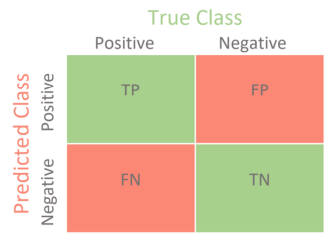
\includegraphics[scale=0.65]{figures/confmat.PNG}
	\caption{Confusion matrix for binary classification\cite{confmat}}
	\label{FigConfMatTF}
\end{figure}

The figure \ref{FigConfMatTF} displays the placement of the described values into a form of confusion matrix. For $n$-labels classification, a type of confusion matrix $C$ that takes into account not only the binary correctness state of prediction (if was right or not), but also the relations between each two labels $i$ and $j$ is illustrated in figure \ref{FigConfMatN}. Here, $C_{i j}$ represents the amount of ${i}$ labeled data that have been classified under label $j$. The metrics above can be generalized, globally or per each label, on this type of confusion matrix:
$$\mathrm{accuracy} = \frac{\sum_{i=1}^n{C_{i i}}}{\sum_{j=1}^n\sum_{i=1}^n{C_{i j}}}$$
$$\mathrm{precision}_i = \frac{C_{i i}}{\sum_{j=1}^n{C_{j i}}}$$
$$\mathrm{recall}_i = \frac{C_{i i}}{\sum_{j=1}^n{C_{i j}}}$$


\begin{figure}[htbp]
	\centering
	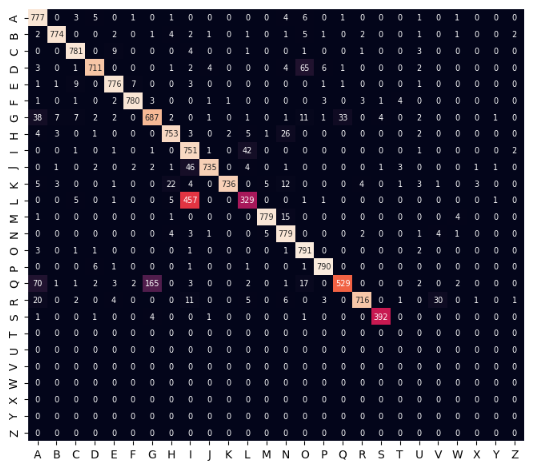
\includegraphics[scale=0.50]{figures/confmat_n.PNG}
	\caption{Confusion matrix for a custom trained EMNIST classification model}
	\label{FigConfMatN}
\end{figure}

\section{Architecture of neural networks}
\label{subsec:ch3sec3}
\subsection{Neural network models}
\label{subsec:ch3sec3subsec1}

A neural network model can be described by a flow graph whose nodes are functions that operates on tensors \cite{Tensorflow}. Such functions are called layers, following the intuition that composing two operations can be imagined as stacking two layers of processing activities. Each layer may use some additional parameters in its operations. They can be either hyperparameters, which are set by the user and define the behavior of the layer, or weights, which are values that reside in an internal state of the layer and can be trainable (updated when a data flow passes through the model) or untrainable (fixed) \cite{Tensorflow}. The weights make the subject of an optimisation problem which ultimately is the powering core of artifical intelligence. The goal is to find the right combination of layers with the weights that best fit a provided problem. The following sections will briefly showcase some of the most popular concepts in deep learning.

\subsection{Multilayer Perceptron}
\label{subsec:ch3sec3subsec2}

The Multiplayer Perceptron (MLP) is the simplest type of neural network. If consists of neurons stacked in multple layers, where each neuron in a certain layer is connected to all the neurons in the following layer \cite{D2l}. There is at least one input layer $i$, one output layer $o$ and a number of hidden layers $h^{i}$ (Figure \ref{FigMLP}). Each layer can be visualised as a uni-dimensional array of neurons that hold a specific value. Each link from a neuron to other carry a weight value \cite{D2l}. 

\begin{figure}[htbp]
    \centering
        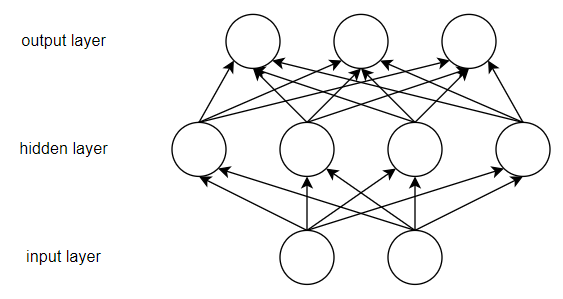
\includegraphics[scale=0.6]{figures/mlp.png}
    \caption{Multilayer perceptron}
    \label{FigMLP}        
\end{figure}

Let's imagine a MLP with the layers $i=h^0, h^1, \cdots, h^n, o=h^{n+1}$. We call $h^{k}_{i}$ be the value of the neuron $i$ from the layer $k$ and $w^k_{i,j}$ the weight of the arc that connects neuron $h^{k}_{i}$ to $h^{k+1}_j$. The forward pass through the MLP can be described using these notation as follows:
$$h^{k+1}_j = \sigma\left(\sum_{i}{w^k_{i,j} h^k_{i}}\right), k=\overline{0,n},$$
where $\sigma$ is an activation function \cite{D2l}. It is easy to find that in matriceal form, this formula can be expressed as $h^{k+1}=\sigma(w^k h^k)$. As it was mentioned in section \ref{subsec:ch3sec2subsec3}, the backward propagation can be automatically derived from the computational graph, therefore it will be omitted in order to focus on other essential concepts.

Without any activation (e.g. when $\sigma(x)=x$), the MLP behaves as a linear map between inputs and outputs. The role of activation function is to allow for covering more complex relationship between the data. 

\subsection{Convolution networks}
\label{subsec:ch3sec3subsec3}

Multilayer perceptrons are particularly costly when it comes to huge volumes of data, and its simplicity can prove detrimental for some types of tasks. Also, they are not designed to work with multidimensional shaped inputs. Sometimes it is useful to add a degree of locality to the relations between neurons \cite{D2l}. This one of the motivations behind the convolutional neural network (CNN) \cite{cnn}. The current section will talk about the 2-dimensional usecase of convolutional networks, although the approach can be generalized to any number of dimensions.

\begin{figure}[htbp]
    \centering
        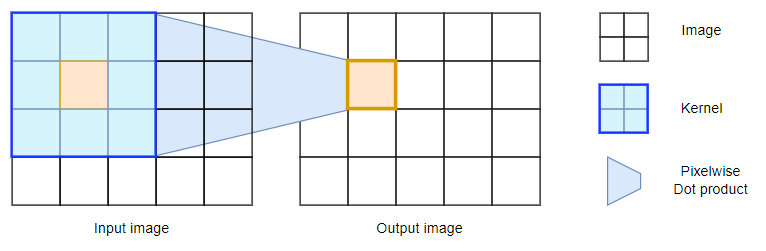
\includegraphics[scale=0.6]{figures/conv2d.PNG}
    \caption{Single channel 3x3 convolution}
    \label{FigConv2D}        
\end{figure}

To give an intuition on the matter, suppose we have an input image $A=(a_{i,j})\in\mathcal{M}_{m,n}(\mathbb{R})$ and a matrix $K=(k_{i,j})\in\mathcal{M}_{2p+1,2q+1}(\mathbb{R})$ called the convolution kernel (Figure \ref{FigConv2D}). Then, the convolution with kernel $K$ applied to the image $A$ is a new matrix $A * K = C=(c_{i,j})\in\mathcal{M}_{m,n}(\mathbb{R})$, where
$$c_{i,j} = \sum_{x=i-p}^{i+p}\sum_{y=j-q}^{j+q} a_{x,y} k_{x-i+1, y-j+1} , $$
where the values at out of bounds indices can be defaulted to $0$ \cite{D2l}. It is the user's choice whether the convolution output dimensions are reduced in order to keep the formula in bounds, or that the input is padded following a custom rule such that the dimensions remain invariant to the operation.

In reality, the 2D convolution operates on multiple matrices of this kind at once, or, in other words, multiple channels of data. Let $A=(a_{i_1,i_2,i_3})\in\mathcal{T}_3((w,h,c_1))$ and $K=(k_{j_1,j_2,j_3,j_4})\in\mathcal{T}_4((2p+1,2q+1,c_1,c_2))$ the convolution kernel. Then, the result of the convolution $A*K = C=(c_{i,j,u})\in\mathcal{T}_3((w,h,c_2))$, where
$$c_{i,j,u}=\sum_{x=i-p}^{i+p} \sum_{y=j-q}^{j+q} \sum_{z=1}^{c_1} a_{x,y,z}\cdot k_{x-i+1, y-j+1,z,u}.$$
This formula to obtain $c_{i,j,u}$ is equivalent to isolating one portion of the input that the kernel overlaps, then perform batch matrix multiplication which changes the number of channels to $c_2$, and finally add the resulted vectors together \cite{D2l}.

Of course, the kernel's width and height is not required to be odd. It was chosen so in order to keep the explanation as simple as possible. In case of an even kernel size, one can note that the center of the kernel visually falls between to elements instead of over one element. In order to perform even-sized kernel convolution, the kernel must be properly aligned over the input via an offset shifting. Instead, a pseudocode has been provided below which performs general kernel multichannel convolution. Note that the algorithms in literature include extra features like striding, dilation or channels-first algorithms \cite{D2l}.

\begin{lstlisting}[language=pascal, escapeinside={(*}{*)}]

function conv2d(a:float[N,M,C], k:float[K1,K2,C,F]) 
{ input: matrix a and convolution kernel k }
{ output: result of convolution a*k = r: float[N,M,F] }
for n, m:=0..N-1, 0..M-1 
  for k1:=0..K1-1
   i := n + k1 - (K1 div 2)
   if not 0<=i<N then continue end
   for k2:=0..K2-1
    j := m + k2 - (K2 div 2)
    if not 0<=j<M then continue end
    for c, f := 0..C-1, 0..F-1     
      r[n,m,f] := r[n,m,f] + a[i,j,c] * k[k1,k2,c,f]
    end
   end
 end 
end
\end{lstlisting}

Note that this approach, although easy to understand, is not the best implementation choice. A faster algorithm is Img2Col, which improves time performance at the cost of memory redundancy while reducing the convolution problem to a matter of matrix multiplication \cite{img2col}. It is also worth mentioning the optimization done by performing the convolution in a Fourier space, which is said to give better results when using larger kernels \cite{fourierconv}.

\subsubsection{Applications in image processing}
\label{subsubsec:ch3sec3subsec3subsubsec1}

The applications of convolutions exceed the boundaries of AI. They are a dependable tool in many graphics manipulations. The image filters offered by real software applications most likely have a convolution behind. Blurs and Canny edge detection \cite{canny} are some common examples of convolution applications in image processing \cite{imgproc}. Some examples of filters are showcased in Table \ref{TabConvImg}. 

\newcommand\cincludegraphics[2][]{\raisebox{-0.3\height}{\includegraphics[#1]{#2}}}

\begin{table}[htbp]
\begin{center}
\begin{tabular}{c c c }
\hline
 Filter name  &  Kernel & Image\\
Identity 
     & $\left( \begin{matrix}1 & 0 & 0 \\ 0 & 1 & 0 \\ 0 & 0 & 1 \end{matrix} \right)$      
     & \cincludegraphics[scale=0.2]{figures/conv_ex_id.png} \\

Sobel X 
     & $ \left( \begin{matrix}1 & 0 & -1 \\ 2 & 0 & -2 \\ 1 & 0 & -1 \end{matrix} \right)$      
     & \cincludegraphics[scale=0.2]{figures/conv_ex_sobelx.png} \\
Sobel Y
     & $ \left( \begin{matrix}1 & 2 & 1 \\ 0 & 0 & 0 \\ -1 & -2 & -1 \end{matrix} \right)$      
     & \cincludegraphics[scale=0.2]{figures/conv_ex_sobely.png} \\
Ridge
     & $ \left( \begin{matrix}0 & -1 & 0 \\ -1 & 4 & -1 \\ 0 & -1 & 0 \end{matrix} \right)$      
     & \cincludegraphics[scale=0.2]{figures/conv_ex_ridge.png} \\
Sharpen
     & $ \left( \begin{matrix}0 & -1 & 0 \\ -1 & 5 & -1 \\ 0 & -1 & 0 \end{matrix} \right)$      
     & \cincludegraphics[scale=0.2]{figures/conv_ex_sharpen.png} \\
\hline
\end{tabular}
\end{center}
\caption{Example of image filters \cite{imgproc}}
\label{TabConvImg}
\end{table}

\begin{figure}[htbp]
    \centering
        
\includegraphics[scale=0.4]{figures/conv_feature_ext.png}
    \caption{Output of the first Conv2D layer in a model trained on MNIST dataset}
    \label{FigConv2D}        
\end{figure}

In deep learning, convolutions are generally used for features extraction. The more filter channels the kernel outputs, the more features the model is able to find, and that many feature maps are generated. A feature map is basically a 2-D slicing through the 3-D output tensor where the index at channel dimension is kept constant. In a convolution layer, the kernels represent the trainable weights. In a convolutional neural network (CNN) architecture, convolutional layers are paired with other layer types (e.g. pooling) in order to achieve maximum performance. A structure of stacked convolution layers can be followed by the previously described fully connected layers in order to give a final touch to the data by bringing it to a requested output shape \cite{cnn}.

\subsubsection{MaxPooling}
\label{subsubsec:ch3sec3subsec3subsubsec2}

As the number of features increases after each convolution layer, the size of the feature maps should decrease in order to keep the memory usage in balance. That explains the need for a volume reducing layer such as the pooling layer. To perform a pooling operation in its simplest form, the input image is partitioned into a number of regions (pools) of a predefined size (pooling size). For each pool, a reduction operation is applied to its elements and the results are recombined to form a new image of a smaller size \cite{cnn}. An example is illustrated in Figure \ref{FigPooling} The type of reduction gives the nature of the layer. Some popular choices are poolings that use the $min$, $max$, or average functions \cite{Tensorflow}. These layers do not have trainable weights, however, it comes to the user's responsibility to find the most suitable pooling size to their problem and other additional configurations like the padding or strides.

\begin{figure}[htbp]
    \centering
        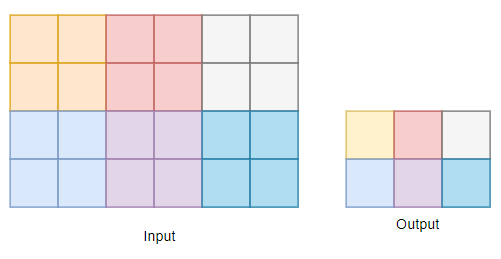
\includegraphics[scale=0.8]{figures/pooling.PNG}
    \caption{Pooling example with 2x2 pool size}
    \label{FigPooling}
\end{figure}

\subsubsection{Dropout}
\label{subsubsec:ch3sec3subsec3subsubsec3}

Overfitting is a subject that will be addressed in a later section in this work. For now, it is relevant to know that during the training process, the weights may become too dependent on the training dataset. This is a issue in a sense that trying to use the model on other types of data may result in noticeable failures. A way to fight overfitting is to cancel (zerorize) a tiny fraction of randomly chosen features at some key points in the training process in order to force the model to generalize its weights in a better way \cite{dropout}.

\subsubsection{LeNet. AlexNet. VGG}
\label{subsubsec:ch3sec3subsec3subsubsec4}

\begin{figure}[htbp]
    \centering
        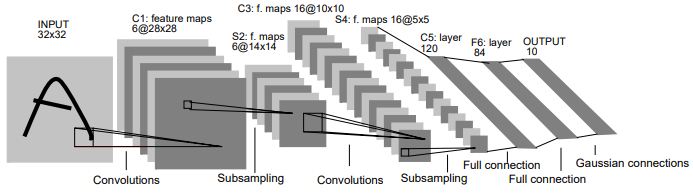
\includegraphics[width=\textwidth]{figures/lenet.PNG}
    \caption{The LeNet-5 architecture \cite{lenet}}
    \label{FigLeNet}
\end{figure}

LeNet (Figure \ref{FigLeNet}) is a basic CNN architecture that serves as a skeleton for other convolutional network applications. It is structured to contain a series of alternating convolution and sub-sampling layers (which was an average pooling in the original architecture) followed by two fully connected layers \cite{lenet}. It was designed to achieve optimal performance on recognizing individual handwritten characters in the MNIST dataset compared to competing methods at the time of introduction, 1998. Since then, LeNet's potential and simplicity secured its position as a template for the following advanced and sophisticated CNN models.

AlexNet is built using convolution, max pooling, dropout and dense layers, with its distinct feature that the workflow is split into two distinct jobs that can be run independently on differnet GPUs. One processing unit runs the first half of the input while the other half is left to second processor. The two work branches are synchronized on the way by letting a convolution layer or dense layers take inputs from both of them, and the results are finally combined and passed through a dense layer to produce a 1000-length Softmax output for image classification purposes \cite{alexnet}.

\begin{figure}[htbp]
    \centering
        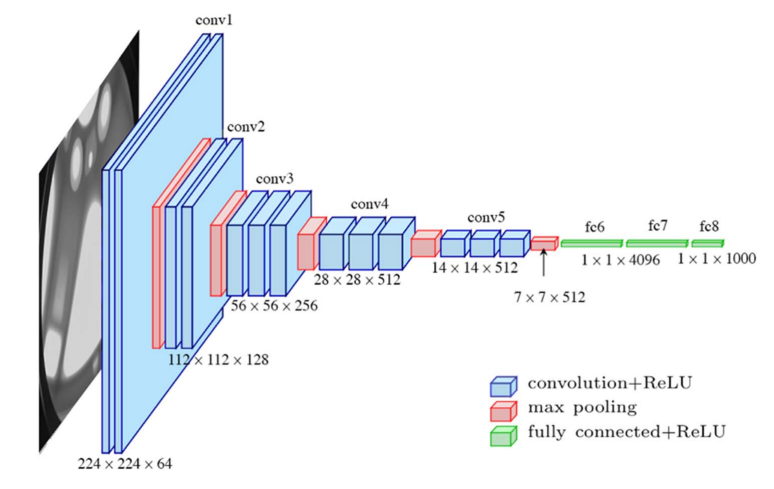
\includegraphics[width=0.7\textwidth]{figures/vgg16.PNG}
    \caption{The VGG-16 architecture \cite{vggpic}}
    \label{FigVGG16}
\end{figure}

Other CNN variants are pushing the depth of the network to greater extends. The VGG model is an example of such a "very deep" architecture. Otherwise structurally similar to common CNNs, it features 16 deep learning layers (there also exists the 19 layers variant) --- see Figure \ref{FigVGG16}. This increased depth allows for more accurate training on larger datasets, but training that large number of parameters in a stable and feasible way requires a bit of delicacy. For this reason, deep models like the VGG are typically subject to fine-tuning, a process in which a pretrained model (for instance, on the ImageNet database) is furtherly trained on the user's end using a target dataset. This approach cuts down training time while making it possible to apply very deep learning techniques on potentially smaller dataset \cite{vgg}.

Furthermore, there exist more complex designs for CNN models. The ResNet improves on the architecture by repumping output from layers behind (residual) into the flow by adding it to the current output \cite{resnet}. In a related fashion, the DenseNet layers can see the entirety of features from all the previous layers \cite{densenet}. Google's Inception network is a carefully optimized architecture which makes use of cleverly placed 1x1 convolutions to reduce the weight count of the model \cite{inception}.

\subsubsection{U-Net}
\label{subsubsec:ch3sec3subsec3subsubsec4}

\begin{figure}[htbp]
    \centering
        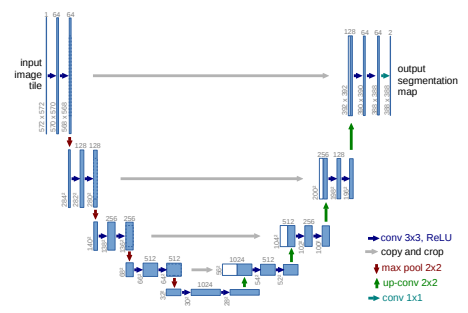
\includegraphics[width=0.7\textwidth]{figures/unet_paper.PNG}
    \caption{The U-Net architecture \cite{vggpic}}
    \label{FigUNet}
\end{figure}

The U-Net was originally engineered for medical applications, therefore it is to be expected that its performance stands up to its fated mission \cite{unet}. It is easyly recognizable by the U letter shape its model schematic resembles, as shown in Figure \ref{FigUNet}. The U-Net is used in per-pixel image segmentation, when an input image is converted to a masked image. As it was previously observed, the flavor of CNNs is feature extraction while reducing the feature map size and extending the channels count. The U-Net builds up on this idea and uses the extracted features to reconstruct a mask image in a process roughly described as an inverse to the convolutional part of the model. A new type of layer, called up-sampling, multiplies the size of the map by copying each feature in a similar way a nearest neighbor resize algorithm rescales an image to one double its size. It is used to reshape the data back to the size of the input while reducing the features depth. An "up-convolution" operation uses upsampling followed by a convolution layer. Then, the model concatenates the output to the feature map of the same size obtained during the feature extraction ("left side" of the U) and convolve the result again, thus completing one step in the mask producing process (the "right side" of the U) \cite{unet}. Another U-Net variant uses transposed convolution with strides of length 2 to replace the up-convolutions \cite{unetconvt}.

\subsubsection{Batch Normalization. Layer Normalization}
\label{subsubsec:ch3sec3subsec3subsubsec5}

Normalization is a crucial step in data processing that gets rid of fluctuations in the dataset that may cause struggles in the training process. Normalization is usually performed at input preprocessing time, however there are cases when one would want a mid-layer normalization step to prevent diverging outputs.

One statistically standard and context independent normalization method is to bring the discrete observation $X=x_1,\cdots,x_n$ to a form $Y$ which has mean $0$ and variance $1$. For that matter, the mean and variance of $X$ are computed: 
$$\mathrm{E}(X) = \frac{1}{n}\sum_{i=1}^{n}x_i, \
\mathrm{Var}(X)= \frac{1}{n}\sum_{i=1}^{n}(x_i-\mathrm{E}(X))^2.$$
Then, the new normalized value $Y$ is obtained as following:
$$ Y = \frac{X - \mathrm{E}(X)}{\sqrt{\mathrm{Var}(X) + \varepsilon}},$$ 
where $\varepsilon$ is a constant included for numerical stability. This formula ensures that $\mathrm{E}(Y)\approx 0$ and $\mathrm{Var}(Y)\approx 1$. Layer normalization is the process that uses this formula on all values of a layer's output \cite{layernorm}.

In the context of $n$-dimensional inputs, one can choose to apply this transformation on a slice of the tensor where the indices of the target axis are kept constant. For example, to normalize each channel in a batched feature maps tensor $X$ of shape $(B, H, W, C)$, $C$ idenependent normalizations are performed on the flattened forms of 3-dimensional tensors $X_{b,i,j,1}, X_{b,i,j,2}, \ldots, X_{b,i,j,C}$. This method is used as a batch normalization technique \cite{batchnorm}.

These batch  normalization layer has different behaviors at train and inference time. When training, the model updates the mean and variance according to the train dataset values and keeps track of them in the form of two parameters, moving mean and moving variance. To obtain a new value of the moving mean when a batch is processed, a weighted mean is computed between its current value and the batch mean with a weight (momentum) selected by the user. It is the same for the moving variance. Two optional parameters $\beta$ and $\gamma$, called offset factor, respectively scaling factor, can learn to linearly transform the mean $0$ - variance $1$ output to a distribution scaled with the factor $\gamma$ and centered in $\beta$. 
At training time, batch normalization uses the real batch mean and variance in normalization. At inference time, the moving mean and variance are used in computations instead of the input batch mean. Neither the mean and variance, nor the factors $\gamma$ and $\beta$ are updated at inference time \cite{batchnorm}.

\subsection{Recurrent neural networks}
\label{subsec:ch3sec3subsec4}

Some problems deal with data that comes in form of sequences. An example is speech recognition, which analyzes sequences of audio frequencies. Other applications imply predicting a fact based of previous observations, as is the case in weather or economy. The length of an input sequence can be arbitrarily long, and patterns may occur during the observed eveniments, therefore is made sense for scientists to come up with a neural network model suitable for this kind of task. The Recurrent Neural Networks (RNN) specialized in processing sequential data \cite{rnn}.

\subsubsection{RNN base model}
\label{subsubsec:ch3sec3subsec4subsubsec1}

A RNN model is conceptually different from other types of networks presented so far in a way that RNN introduces cycles in the information flow by using its own outputs as inputs. RNN runs one cycle for each item contained in a sequence. At each step, a hidden state of the network is computed which is then fed into the RNN on the next cycle, along with the next element in the input sequence  \cite{rnn}. The recurrence can be easily demystified by unfolding the network in order to transform the cycle into a linear flow, as shown in Figure \ref{FigRNN} \cite{rnn_cells_pic}. 

\begin{figure}[htbp]
    \centering
        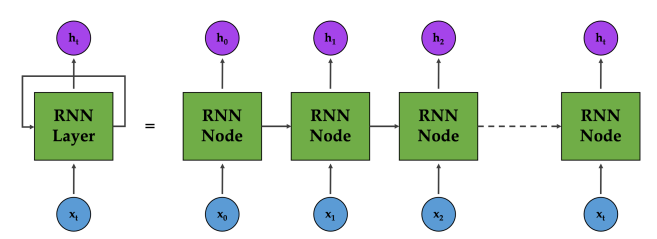
\includegraphics[width=0.7\textwidth]{figures/rnn_layer.PNG}
    \caption{RNN layer and its unfolded representation \cite{rnn_cells_pic}}
    \label{FigRNN}
\end{figure}

Let $T\in\mathbb{N}$ be a number of timestamps and $\mathrm{X} = (\mathrm{x}_1, \ldots, \mathrm{x}_T) \in \mathcal{T}((T, D))$ a sequential input of $T$ elements represented as $D$-length vectors. Let $\mathrm{h}_t \in \mathcal{T}((U))$ be the hidden state of the RNN having length $U$. For starters, $\mathrm{h}_0 = 0$. At a timestamp $t=\overline{1,T}$, the RNN finds $\mathrm{h}_t$ in terms of $\mathrm{x}_t$ and $\mathrm{h}_{t-1}$ using the following recurrent relationship:
\begin{gather}
 \mathrm{h}_t = \sigma_h ( W^{xh} \mathrm{x}_t + W^{hh} \mathrm{h}_{t-1} + b_h), 
 \end{gather}
where $W^{xh} \in \mathcal{T}((D, U)), W^{hh} \in \mathcal{T}((U, U))$ are weights, $b_h \in \mathcal{T}((U))$ is the bias and $\sigma_h$ is a recurrent activation function \cite{rnn}. Along the hidden state, which is reserved for internal use, an output $\mathrm{O}=(\mathrm{o}_1,\ldots,\mathrm{o}_T)$ is computed in a similar fashion using the previous result $\mathrm{h}_t$:
\begin{gather} \mathrm{o}_t = \sigma_o(W^{ho} \mathrm{h}_t + b_o). \end{gather}
Usually, the activation function can be tanh or sigmoid \cite{rnn}.

By isolating the mechanism that computes the hidden states and the output, one would obtain what is called a RNN cell, which makes it easier to visualize the inner workings of the RNN. It also helps clearly separate the recurrent step in the cell from the entire RNN model( which at the end of the day is calling the cell acting like a zipper machine on the input and hidden sequences) \cite{rnn}. A pseudocode for a generic RNN forward propagation is provided below.
\begin{lstlisting}[language=pascal, escapeinside={[*}{*]}]
function rnn_forward_pass(x, cell)
{ input:  x, a sequencial input of T elements   }
{         cell, the RNN cell in functional form }
{ output: o, a sequence of T outputs            }
  h[*$_0$*]=0
  for t:=1..T do
    h[*$_t$*], o[*$_t$*] = cell(x[*$_t$*], h[*$_{t-1}$*])
  end
end
\end{lstlisting}

 It was observed that the RNN produces a sequence of $T$ outputs. The programmer has the choice to remember only the last computation, which may be interpreted as predicting the value at timestamp $T+1$, or keep the entire sequence of outputs. 

Note that the RNN cell can contain more complex logic, which consequently leads to more performant models. Two of them will be mentioned in the next sections. Visual representations of RNN cells are shown in Figure \ref{FigRNNCells}.

\subsubsection{Long-Short Term Memory}
\label{subsubsec:ch3sec3subsec4subsubsec2}

Is was observed that the RNN faces training issues caused by the vanishing or exploding gradient which affect the model'a ability to handle long term dependencies \cite{rnn_gradient_problems}. While huge values of gradient can be naively fixed by manually clipping it up to a maximum threshold, the vanishing gradient problem, which describes the situation of loss rapidly converging to $0$, is a bit tougher to address \cite{rnn_gradient_problems}. 

\begin{figure}[htbp]
    \centering
        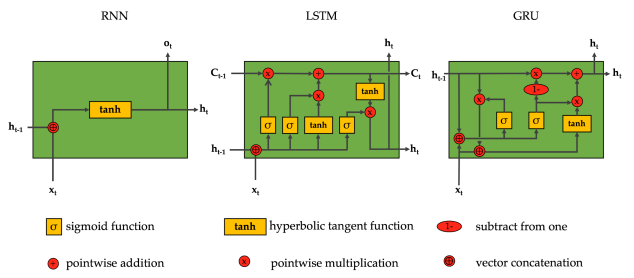
\includegraphics[width=0.7\textwidth]{figures/rnn_cells.PNG}
    \caption{Internal workings of RNN, LSTM and GRU cells \cite{rnn_cells_pic}}
    \label{FigRNNCells}
\end{figure}

For that matter a new type of RNN cell was introduced. The Long-Short Term Memory (LSTM) was proposed as a solution to the vanishing gradient problem. Due to their error stability, LSTM units are able to keep track of dependencies over a wider range of timestamps \cite{rnn}. LSTM features an additional memory mechanism which is controlled by three gates. An input gate ($\mathrm{I}$) filters the input to be stored into the cell's memory, while an output gate ($\mathrm{O}$) chooses the most relevant information to be passed to the next step \cite{lstm}. A forget gate ($\mathrm{F}$) makes the memory lose possibly unwanted information \cite{rnn}. The output of these gates are computed in a similar fashion there has been seen above:
\begin{gather}
\mathrm{I}_t = \sigma ( W^{xi} \mathrm{x}_t + W^{hi} \mathrm{h}_{t-1} + b_i) \\
\mathrm{O}_t = \sigma ( W^{xo} \mathrm{x}_t + W^{ho} \mathrm{h}_{t-1} + b_o) \\
\mathrm{F}_t = \sigma ( W^{xf} \mathrm{x}_t + W^{hf} \mathrm{h}_{t-1} + b_f),
\end{gather}
where $\sigma$ denotes the sigmoid function \cite{rnn}.

The memory content is noted $C$. Before that, a candidate memory $\tilde{C}$ is calculated:
\begin{gather}
\tilde{\mathrm{C}}_t = \tanh ( W^{xc} \mathrm{x}_t + W^{hc} \mathrm{h}_{t-1} + b_c),
\end{gather}
which in amplified by the input gate and added to the cell's memory decaying content according to the forget gate \cite{rnn}:
\begin{gather}
\mathrm{C}_t = \mathrm{F}_t \circledcirc \mathrm{C}_{t-1} +  \mathrm{I}_t \circledcirc \tilde{\mathrm{C}}_t.
\end{gather}
Finally, the hidden state is obtained implying the output gate and the freshly updated memory:
\begin{gather}
\mathrm{H}_t = \mathrm{O}_t \circledcirc \tanh(\mathrm{C}_t),
\end{gather}
thus completing a LSTM cell forward step \cite{rnn}. The hidden also serves as the effective output of the cell.

Another variant of this cell is the peephole LSTM design, which tries to use the cell memory to produce the input, output and forget gates results \cite{peephole_lstm}. There is also the Gated Recurrent Unit (GRU) which shares common points with the LSTM, although it uses only two gates (update and reset) with no output gate, thus having less weights, which makes them easier to train, while still keeping the effectiveness comparable to the one of LSTM \cite{gru}. 

\subsubsection{Encoder-decoder model}
\label{subsec:ch3sec3subsec4}

The encoder-decoder is a simple and flexible neural network template which consists of two phases: an encoder takes an input of some sort and produces a vector of features, then a decoder uses that vector to obtain an output \cite{rnn}. when the input and the output are identical, the model is called autoencoder and is useful in compressing the data by finding the most compact way to store deatures into the limited size intermediate vector \cite{autoencoder}. An interesting application of this concept is the Variational Autoencoder (VAE), where slightly altering the encoded vector in the continuous space makes it capable of creational tasks \cite{autoencoder}. When the encoder-decoder has input and output in sequential form, it is called a sequence-to-sequence model (seq2seq) \cite{rnn}.

\subsubsection{Connectionist Temporal Classification}
\label{subsec:ch3sec3subsec4subsubsec4}

Sequene-to-sequence classification problems involve associating a label to each item in an input sequence. For example in the speech recognition problem, an audio to text formulation may sound like this: the input is divided into $T$ small sound units (which may go as low as the recording hardware precision), and for each unit a model tries to predict the phonem which is in the course of spelling. The key observation is that a single phonem can be pronounced during any number of consecutive timestamps, making it impossible for such a mathematical model to make one to one connections between audio units and letters in a word. For example, if the input is a recording of the word "cat", a possible classification output sequence with 9 timestamps may look like "cccaaaatt" \cite{ctc_loss_explained}. This situation encourages the intuition to concatenate identical labels into one single output element, in order to obtain the correct word. However, this approach generates confusion in case of words containing duplicate letters. For instance, in a pronounciation of the word "steel" which produces the sequence of classes "sstteeell", the above logic would output the string "stel", since there is not enough information about how many adjacent "e"s there actually are, or which part of the labels sequence corresponds to the first or the second "e". This is the point there an approach called \mbox{Connectionist Temporal Classification} (CTC) comes in handy when labels are spread accross multiple timestamps \cite{ctc}. 

\begin{figure}[htbp]
    \centering
        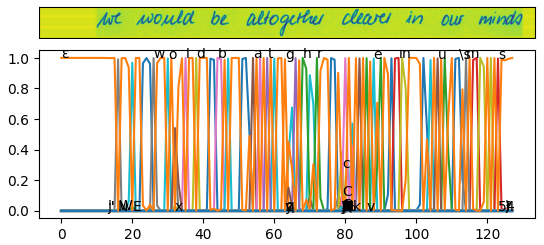
\includegraphics[width=0.7\textwidth]{figures/ctc_on_htr.png}
    \caption{CTC probabilities in a HTR context (IAM dataset sample)}
    \label{FigCTC}
\end{figure}

Let $L$ be a the of labels of interest. The CTC adds an extra label $\varepsilon$ to the output called the blank label to define the absence of an observation \cite{ctc}. Now, suppose an input $\mathrm{x} \in \mathcal{T}((T, n))$ generates a sequence of softmax probabilities $\mathrm{y} \in \mathcal{T}((T, m))$ (Figure \ref{FigCTC} displays the sequence of character probabilities generated by a HTR model). Let $\pi\in(L\cup\{\varepsilon\})^T$ be a sequence of labels. For simplicity, the labels are seen as a subset of natural numbers: $L=\{1,2,\ldots,|L|\}\subset \mathbb{N}$ and the extra label will be assigned the number $\varepsilon=|L|+1$. CTC defines the probability of the labels path $\pi$ when input $\mathrm{x}$ produces the sequence of probabilities $\mathrm{y}$:
$$ p(\pi|\mathrm{x}) = \prod_{t=1}^T \mathrm{y}_{t, \pi_t} \ \cite{ctc}. $$

Then, the set of all possible sequence of labels of length not greater than $T$ (called labellings) is defined as $L^{\leq T} = \{ (l_1\ldots l_k)\ | \ l_i\in L, 1\leq i\leq k\leq T \lor k=0 \}$ along with an operator $\mathcal{B}:(L\cup\{\varepsilon\})^T\rightarrow L^{\leq T}$ that extract the final output sequence from a path by removing the adjacent duplicate labels and blank labels, in this exact order \cite{ctc}. The inverse image of this operator, 
$\mathcal{B}^{-1}$, for an $l\in L^{\le T}$, is the set of paths $\pi$ for which $\mathcal{B}(\pi)=l$. With this in mind, the probability of a an occurring labelling $l\in L^{\leq T}$ is by definition
$$ p(l|\mathrm{x}) = \sum_{\pi\in\mathcal{B}^{-1}(l)} p(\pi|\mathrm{x}), $$
the sum of probabilities of all paths that collapse to $l$ \cite{ctc}.

The goal is to find the labelling $l$ that has the maximum probability: 
$$\mathrm{arg} \max_{l\in L^{\leq T}} p(l|\mathrm{x}) \cite{ctc}.$$ 

This fact, if transformed into a searching problem, can be approached using ideas from dynamic programming. A faster alternative is to have a greedy algorithm build the path $\pi^0=(l_1,\ldots,l_T)$, where $l_t=\mathrm{arg} \max_{i} \mathrm{y}_{t,i}$ \cite{ctc}.

The CTC loss function, 
$$ loss = -\log p(l|\mathrm{x}), $$
is a direct consequence of the idea that minimizing the loss 
leads to the optimal solution (in our case, a maximum probability) \cite{ctc_peaky}.

\subsection{Optimizers}
\label{subsec:ch3sec3subsec6}

As it was previously discussed, deep learning thought as an optimzation problem requires minimizing the loss function. Expressing a neural network as a closure function  $y=\phi_w(x)$ in terms of the weights $w$, where $x, y$ are fixed input-output pairs, minimizing the loss means finding the values of $w$ such that $f(w) = loss(y, \phi(w,x))$ is as low as possible. The algorithm that achieves this is called an optimizer \cite{D2l}.

Gradient descent is an optimization technique based on the derivative (gradient) of the objective function. It starts from the Taylor expansion
$$f(w+e) = f(w) + e^T \nabla f(w) + O(||e||^2),$$
in which the substitution $e=-\eta \nabla f(w)$ is made, where $\eta\in\mathbb{R}$ is a small positive number called the learning rate \cite{D2l}. When $\eta$ is small enough, the term $O(||e||^2)$ becomes negligible, and because $\nabla f(w)^T \nabla f(w)$ contains only positive elements, the expression $ f(w) - \eta \nabla f(w)^T \nabla f(w)$ is guaranteed to decrease: 
$$ f(w-\eta\nabla f(w)) \lessapprox f(w). $$ 
Thus, by repeatedly plugging $w\leftarrow w-\eta \nabla f(w)$ into the formula may converge to a local optimum \cite{D2l}.

In real applications, the loss function is computed accross multiple samples in the dataset: $f_i(w)=loss(y_i, \phi(w, x_i)$ and the training loss is an average of these values: 
$$f(w)=\frac{1}{n}\sum_{i=1}^{n} f_i(w)$$. 
It is remarkable that computing the gradient $\nabla f(w)=\frac{1}{n}\sum_{i=1}^{n} \nabla f_i(w)$ for each iteration has linear $\Theta(n)$ time complexity, where $n$ is the number of samples in the dataset. A workaround to this issue would be at each iteration to choose a uniform random index $i$ and update the weights following the rule 
$$w\leftarrow w-\eta \nabla f_i(w).$$
This method is known as the Stochastic Gradient Descend (SGD), which is a faster and pretty good approximation of the gradient descend  \cite{D2l}. As the gradient descend is applied per sample and SGD on the whole dataset, there also exists a hybrid method when the weights are updated after processing batches of items from the dataset. 

So far the learning rate was assumed to be constant, however, it may be useful to let it vary along epochs, especially when the gradient becomes that small that the learning rate is big enough to prevent the alorithm from optimizing further. The solutions are using a learning rate scheduler $\eta(i)$ in terms of the epoch $i$, or use a more advanced optimizer like RMSProp, Adagrad or Adam, which are able to adapt the learning rate depending on the magnitude of the gradients \cite{D2l}. 

\subsection{Training neural networks}
\label{subsec:ch3sec3subsec7}

So far the focus was on visiting the mathematical tools and deep learning models that left a footprint on the success of artificial intelligence. However, the dataset quality is as important as the architecture itself, therefore a good training should use the dataset in a wise way. This section aims to briefly summarize some relevant techniques used in supervised learning.

\subsubsection{Train data. Validation data. Test data}
\label{subsubsec:ch3sec3subsec7subsubsec1}

It is important to remember that a dataset is only a sampled subset that represents a problem, and real world occurences may still contain rare patterns that are not fully covered in the selection of samples. The fact that an AI model is able to learn the target dataset does not guarantee that it will perform well on all real applications. For this reason, interest must be put into detecting and measuring the robustness of the model when facing never before seen data. Therefore, it is a common practice to partition the data set into two disjoint subsets. A train set is used for effectively training the model, while a validation test is queried at the end of each epoch in inference mode to check performances on. This way, the purpose of the training shifts to improving results on the validation set \cite{data_col}. After the entire training process completes, another test dataset can be used to evaluate the model \cite{train_val_test}. There are of course alternative methods like cross-validation, which happens when the dataset is split into multiple subsets, and at a time some of them serve as training data, while others are validation data. At the end of an interations, the subsets may switch their roles. For exmaple, in $K$-fold cross-validation, each of the $K$ subsets are used in order as a validation set, while the other $K-1$ become training data \cite{train_val_test}. As an additional note, the train validation split needs precaution to prevent training from losing track of some features of classes because most of the samples containing them have been placed in the validation dataset \cite{train_val_test}.

\subsubsection{Overfitting. Underfitting}
\label{subsubsec:ch3sec3subsec7subsubsec5}

Overfitting refers to the phenonemon when the model's ability to generalize is constrained by the excessive number of parameters compared to the volume of trained data \cite{overfitting}. The model tends to learn the dataset "by heart" and does not pay attention anymore to input-output relationship, resulting in worse performance on the validation data. Being such a wide in problem in deep learning, there exist multiple tools (regularizers) to counterattack overfitting \cite{overfitting}. Dropout has already been presented in section \ref{subsubsec:ch3sec3subsec3subsubsec3}.
Hyperparameter tuning may also be an adjuvant factor in this situation \cite{overfitting}, as well as weight decay is, which involves optimizing the weights with respect to a regularization loss (called L1 or L2, which are basically other names for MAE and MSE losses). By keeping the weight as low as possible, weight regularization prevents the model from favorizing a certain feature, thus improving the room for generalization \cite{weight_decay}.

On the other hand, it is said that the model underfits if it performs badly on the training set. A simple explatation for underfitting is that the model needs more training or is too small or too barebones to learn the desired dataset, like using a linear function to fit points on a parabola. Making the model bigger, training for more epochs, or switching to another architecture are some solutions to prevent underfitting. Underfitting is also possibly caused by the poor quality of the dataset \cite{overunderfitting}. 

\subsubsection{Data augmentation. Generators}
\label{subsubsec:ch3sec3subsec7subsubsec2}

Smaller dataset can be artificially grown through the process of data augmentation. Some models may need more training data than available, and programatically enriching a dataset is cheaper and more efficient that manually collecting and labelling more samples. By exposure to augmented data, the model can make abstraction of redundant features and learn the invariants on the datasets. For instance, let's consider an image dataset for object recognition that only contains pictures of centered and horizontally aligned objects. Trained only on such data, the model during testing may not recognize even the exact same object is it was slightly misaligned, rotated or reflected another light intensity. If the dataset is augmented to also include rotated, scaled, translated or constrast altered images obtained from the base dataset, the model's accuracy on variate types on input may significantly increase. This can go way further and add even noise or other impediments to the images. It is a good choice to pair data augmentation with custom forms of training, like for example letting the model learn the easier samples first and then progressively feeding it with more and more interesting augmented images \cite{augmentation}. 

Data augmentation could be a memory intensive process due to the volume of additional data it provides. A fix to this issue is generating augmented data on the fly instead of storing precomputed forms of it. This even allows for infinite sample generation starting from a base database. Tensorflow has great support for dataset generation and iterating \cite{Tensorflow}.

\subsubsection{Data preprocessing}
\label{subsubsec:ch3sec3subsec7subsubsec3}

The quality of model training can be improved by simply showing it information from another angle. Although the concept of preprocessing refers to the greater picture from fetching the dataset from a storage support (be it CSV, database, binary files) up until passing it to the model \cite{D2l}, this section focuses on the step of data normalization. Observing statistical and mathematical patterns in the dataset may lead to apply functions that alter the mean and standard-deviation, create uniform bounds, linearize exponential input and the list continues. The Mean-Centered, Z-Score, Min-Max, Sigmoidal Normalization are examples of normalization methods \cite{normalization}. The reasoning of normalization may also be influenced by the computational precision: the floating point mechanism itself offers a good clue that rounding errors are minimized when working with lower numbers. This is why it is clever to scale (and offset) RGB pixel values from $[0,255]$ to $[0,1]$ or $[-1,1]$. Furthermore, sometimes the features can be more clearly observed in different representation of the same information. For example, when an AI problem needs tonal information about the colors, training complexity could be significantly cut down if images are presented in HSV rather than RGB channelling format \cite{pixel_norm}.


\chapter{Offline handwritten text recognition}
\label{chap:ch3}

\par Lorem ipsum dolor sit amet

\section{Related work}
\label{subsec:ch3sec2subsec1}

\subsection{Hidden Markov Models}
\label{subsec:ch3sec2subsec1subsubsec1}

\subsection{CNN-RNN Networks}
\label{subsec:ch3sec2subsec1subsubsec2}

\subsection{Multi-Dimensional LSTM}
\label{subsec:ch3sec2subsec1subsubsec3}

\subsection{Transformer models}
\label{subsec:ch3sec2subsec1subsubsec4}

\section{Datasets}
\label{subsec:ch3sec2subsec2}

\section{Preprocessing. Segmentation}
\label{subsec:ch3sec2subsec3}

\section{Proposed approach}
\label{subsec:ch3sec2subsec4}

\subsection{Line segmentation model}
\label{subsec:ch3sec2subsec4subsubsec1}

\subsection{Text recognition model}
\label{subsec:ch3sec2subsec4subsubsec2}

\subsection{Dataset}
\label{subsec:ch3sec2subsec4subsubsec3}

\subsection{Used method description}
\label{subsec:ch3sec2subsec4subsubsec4}

\subsection{Results}
\label{subsec:ch3sec2subsec4subsubsec5}

\subsection{Other attempts}
\label{subsec:ch3sec2subsec4subsubsec6}



\chapter{LillyScan - Practical HTR application prototype}
\label{chap:ch4}

\par Lorem ipsum dolor sit amet

\section{Functionalities. Requirements analysis}

\section{Software Design}

\subsection{Usecase diagrams}
\subsection{Conceptual model}
\subsection{Dynamic model}

\section{Implementation. Technical documentation}


\subsection{C\# programming language. .NET framwework}
\label{sec:ch3sec1}

\par Lorem ipsum dolor sit amet


\subsection{Xamarin. MAUI}
\label{subsec:ch3sec2}

\subsection{Object Oriented Programming}
\label{subsec:ch3sec2}

\subsection{Porting the neural network into native language}
\label{subsec:ch3sec2}

\subsection{Deserialization of Python dictionaries}
\label{subsec:ch3sec2}

\section{Application testing and validation}
\chapter{Future work}
\label{chap:ch4}


\chapter{Conclusions}
%\chapter*{Concluzii}
\label{conclusions}

\par Concluzii ...

%\addcontentsline{toc}{chapter}{Concluzii}
%\addcontentsline{toc}{chapter}{Conclusions}

\bibliography{references}

\end{document}
